%%%%%%%%%%%%%%%%%%%%%%%%%%%%%%%%%%%%%%%%%%%%%%%%%%%%%%%%%%%%%%%%%%%
%%% Documento LaTeX 																						%%%
%%%%%%%%%%%%%%%%%%%%%%%%%%%%%%%%%%%%%%%%%%%%%%%%%%%%%%%%%%%%%%%%%%%
% Título:		Capítulo 2
% Autor:  	Ignacio Moreno Doblas
% Fecha:  	2014-02-01
% Versión:	0.5.0
%%%%%%%%%%%%%%%%%%%%%%%%%%%%%%%%%%%%%%%%%%%%%%%%%%%%%%%%%%%%%%%%%%%
\chapterbegin{Implementación}
\label{chp:Impl}
%\minitoc

\section{Análisis de requisitos}
\label{sec:Requirements}

Para el desarrollo de este proyecto se han tenido en cuenta una serie de requisitos previos mínimos, necesarios para una correcta implementación del mismo. Los requisitos funcionales del sistema pueden ser divididos en 2 categorías, dependiendo si nos referimos a la aplicación Android o Web, y fueron acordados en los siguientes:

\subsection{Requisitos funcionales}

\subsubsection{Aplicación Android}

\begin{itemize}
	
\item Capacidad de detectar sensores \ac{BLE} próximos al dispositivo

La aplicación Android debe ser capaz de escanear y detectar cualquier sensor BLE que se encuentre dentro del radio de alcance del dispositivo Android, mostrando su nombre y dirección \ac{MAC} en pantalla.

\item Capacidad de conectarse a cualquier sensor BLE registrado.

La aplicación Android debe ser capaz de establecer una conexión GATT cliente-servidor, mostrando en pantalla los servicios y características ofrecidas por el sensor.

\item Capacidad de leer características GATT ofrecidas por el sensor.

La aplicación Android debe ser capaz de interpretar la información proporcionada por un sensor de ritmo cardíaco o pulsómetro comercial, pudiendo determinar entre otros, la frecuencia cardíaca del usuario o el porcentaje de batería restante.

\item Capacidad de determinar la posición del dispositivo

La aplicación Android debe de ser capaz de determinar la posición geográfica del dispositivo, en términos de latitud y longitud.

\item Capacidad de enviar los parámetros relevantes a través del protocolo HTTP a nuestro servidor web.

La aplicación Android debe ser capaz de enviar valores de frecuencia cardíaca y  localización al servidor web implementado, a través de solicitudes tipo POST del protocolo HTTP.

\end{itemize}

\subsubsection{Aplicación Web}

\begin{itemize}
	
\item Capacidad de determinar si el pulsómetro está conectado al sistema

La aplicación Web deberá reflejar en todo momento si el pulsómetro se encuentra conectado al sistema y emitiendo datos, o si este se encuentra desconectado.

\item Capacidad de mostrar la frecuencia cardíaca actual en tiempo real

El servidor web permanecerá a la escucha de peticiones POST efectuadas por la aplicación puente Android. Estas peticiones contendrán el último valor leído de frecuencia cardíaca y serán inmediatamente transmitidas al cliente web (cualquier navegador) a través de una conexión web socket. El navegador por tanto mostrará en pantalla el último valor recibido mediante una etiqueta numérica.

\item Capacidad de mostrar la evolución de la frecuencia cardíaca mediante el uso de una gráfica dinámica

La aplicación web será capaz de retener un cierto número de valores pasados (dependiendo del tamaño de la pantalla en al cual realizamos la visualización), junto con el valor actual y mostrará dichos valores en una gráfica lineal, la cual dará la sensación de avanzar en el tiempo conforme nuevos valores llegan al cliente web a través de la conexión web socket.

\item Capacidad de guardar los datos de frecuencia cardíaca en una base de datos

El servidor web implementado almacenará cada valor recibido en una base de datos no relacional, reflejando la fecha exacta en la cual tuvo lugar dicha muestra. Esto facilita la futura consulta de valores en ciertos rangos de tiempo para así permitir la posible realización de gráficas y estadísticas a tal efecto.

\item Capacidad de determinar la posición del usuario usando el servicio de mapas de Google

La aplicación web debe ser capaz de mostrar en todo momento la localización del usuario haciendo uso del pulsómetro.

\item Capacidad de notificar por e-mail a un grupo de usuarios interesados en realizar tareas de monitorización

Cuando el valor de ritmo cardíaco sobrepase un cierto rango, se enviará una notificación por e-mail alertando de condiciones anormales, junto con la localización actual del usuario usando el pulsómetro y se mantendrá al interesado o grupo de interesados informado con actualizaciones frecuentes, hasta la que la situación vuelva a la normalidad.

\item Capacidad de adaptarse fácilmente a pantallas más pequeñas, tales como teléfonos móviles y tabletas

La aplicación debe ser \tit{web responsive} y amigable para el usuario en cualquier tipo de pantalla.
 
\end{itemize}

\subsection{Requisitos no funcionales}

Adicionalmente, los siguientes requisitos no funcionales fueron considerados, refiriéndose a la Aplicación como el conjunto Android + Web.

\begin{itemize}
\item Extensibilidad futura.
La aplicación debe de ser fácilmente extensible en un futuro. Para ello se tendrá en mente la modularidad y el código autoexplicativo durante el desarrollo de la aplicación 

\item Tolerancia a fallos.
La aplicación debe de tolerar pequeños fallos sin que estos entorpezcan en medida alguna la posible medición en curso.

\item Rendimiento.
La aplicación no debe de ser una carga importante para el rendimiento del sistema, ya que esto podría resultar en mediciones imprecisas o pérdida de muestras por incapacidad del sistema de copar con la carga.

\item Usabilidad.
La aplicación no debe presentar un dificultoso manejo de cara al usuario.

\end{itemize}

\subsection{Diseño de la interfaz gráfica}

Como paso previo a la implementación en código, se han diseñado unos borradores de las distintas pantallas de las que constará la aplicación, tanto web como Android.

\subsubsection{Android}
La aplicación se ha dividido en cuatro pantallas básicas: reposo, búsqueda, desconectado y conectado, las cuales se pueden observar en las figuras \ref{fig:mockup:reposo}, \ref{fig:mockup:busqueda},  \ref{fig:mockup:desconectado} y \ref{fig:mockup:conectado} respectivamente:

\begin{figure}[h] \centering
\begin{minipage}{0.45\textwidth}\centering
 \includegraphics[height=12cm]{graphs/mockup_android_initial_es.png} \caption{Bosquejo Android estado Reposo}\label{fig:mockup:reposo}
\end{minipage}\hfill
\begin{minipage}{0.45\textwidth}\centering
   \includegraphics[height=12cm]{graphs/mockup_android_searching_es.png} \caption{Bosquejo Android estado Búsqueda}\label{fig:mockup:busqueda}
 \end{minipage}
\end{figure}

\begin{figure}[h] \centering
	\begin{minipage}{0.45\textwidth}\centering
		\includegraphics[height=12cm]{graphs/mockup_android_device_es.png} \caption{Bosquejo Android estado Desconectado}\label{fig:mockup:desconectado}
	\end{minipage}\hfill
	\begin{minipage}{0.45\textwidth}\centering
		\includegraphics[height=12cm]{graphs/mockup_android_emitiendo_es.png} \caption{Bosquejo Android estado Conectado}\label{fig:mockup:conectado}
	\end{minipage}
\end{figure}

\begin{description}
\item Reposo\hfill \\
Representa la primera actividad que será cargada en primer plano cuando lancemos la aplicación. Para empezar a escanear dispositivos dentro del alcance de nuestro teléfono debemos pulsar el botón situado en la barra de acción superior, cuyo icono es el logotipo de Bluetooth.
\item Búsqueda\hfill \\
Muestra una lista con los dispositivos sensores BLE encontrados, en particular el nombre y dirección \ac{MAC} del dispositivo. Para obtener información de cualquiera de los sensores, debemos pulsar el elemento correspondiente en la lista. Esto nos llevará a la actividad de perfil del dispositivo, en principio en su estado \tit{desconectado}.
\item Desconectado\hfill \\
 Muestra una interfaz gráfica básica para la monitorización de la conexión, junto con la dirección \ac{MAC} del sensor. Para conectarnos al dispositivo debemos pulsar en el botón conectar situado en la barra de acción superior. Una vez que la conexión Bluetooth ha sido establecida, la interfaz de usuario cambiará a su estado \tit{conectado}.
\item Conectado\hfill \\
 Muestra una lista expandible de los servicios ofrecidos por el sensor. Para consultar las características que un servicio en particular contiene, debemos pulsar en dicho elemento de la lista y esto hará que se expandan las características disponibles. Para empezar a recibir datos del sensor debemos pulsar en cualquier característica, lo que actualizará el campo ``datos'' de la actividad mostrando el valor recibido. Mediante el pulsado de la característica ``Medida de la Frecuencia Cardíaca'' activaremos e instanciaremos el cliente HTTP para así comenzar a enviar valores de ritmo cardíaco en tiempo real y la localización geográfica del usuario a nuestro servidor web mediante solicitudes de tipo POST y la aplicación podrá seguir funcionando en segundo plano, hasta que decidamos desconectar.
\end{description} 

\subsubsection{Web}
La aplicación web presenta dos estados básicos en cuanto a la interfaz gráfica se refiere, que son desconectado y conectado,  las cuales pueden contemplarse en las figuras \ref{fig:mockup:web:desconectado} y \ref{fig:mockup:web:conectado} respectivamente. Si la aplicación Android se encuentra en estado \tit{conectado}, la aplicación web automáticamente se encontrará en estado \tit{conectado} mostrando una gráfica con los últimos valores recibidos junto con el valor actual. El resto de posibles estados de la aplicación Android se corresponderán con el estado \tit{desconectado} de la aplicación web.

\begin{figure}[h] \centering
	\includegraphics[width=15cm]{graphs/mockup_web_disconnected_es.png} \caption{Bosquejo web con sensor desconectado}\label{fig:mockup:web:desconectado}
\end{figure}

\begin{figure}[h] \centering
	\includegraphics[width=15cm]{graphs/mockup_web_connected_es.png} \caption{Bosquejo web con sensor conectado}\label{fig:mockup:web:conectado}
\end{figure}

El botón con etiqueta ``Localización del usuario''  nos redirigirá al servicio de mapas de Google mostrando la localización del poseedor del sensor en ese preciso instante y estará habilitado unicamente si nos encontramos en el estado \tit{conectado}.


\subsection{Dispositivo Android}
    El desarrollo de este proyecto ha sido realizado y probado en un Google Nexus 5, bajo la versión Android 5.0, lo cual garantiza que la aplicación conserva toda su funcionalidad en los modelos más modernos, tanto en software como en hardware. 
    
    La versión mínima de Android requerida para el correcto funcionamiento de esta aplicación, es el nivel de \ac{API} 18, correspondiente a Android 4.3, ya que es la primera versión que incorpora soporte para BLE.

\section{Aplicación Android}

\subsection{Entorno de desarrollo integrado}
\label{sec:IDE}
\begin{figure}[h] \centering
    \includegraphics[width=15cm]{graphs/android_studio.png} \caption{Entorno de desarrollo integrado Android Studio}\label{fig:astudio}
\end{figure}
 \begin{figure}[h] \centering
    \includegraphics[width=15cm]{graphs/eclipse.png} \caption{Entorno de desarrollo integrado Eclipse}\label{fig:eclipse}
\end{figure}
    Es posible elegir entre varios entornos integrados de desarrollo a la hora de desarrollar una aplicación para la plataforma Android. Los dos principales son Eclipse y Android Studio.
    
    Android Studio es un \ac{IDE} específico para desarrollar en la plataforma Android. Está basado en el popular IntelliJ IDEA de la compañía JetBrains, pero fuertemente modificado, tanto en aspecto como en funcionalidad. Android Studio es de reciente desarrollo, llegando a su versión 1.0 inicial en Diciembre de 2014. La versión 1.0.2 se puede observar en la figura \ref{fig:astudio}.

    Eclipse es un \ac{IDE} de propósito general, que provee un espacio de trabajo y un sistema de complementos muy extensible y flexible. Está escrito en Java, e inicialmente se enfocó al desarrollo en dicho lenguaje. 
    
    Gracias a su sistema de complementos, Eclipse puede ser utilizado para desarrollar aplicaciones en múltiples lenguajes: Ada, ABAP, C, C++, COBOL, Fortran, Haskell, JavaScript, Lasso, Lua, Natural, Perl, PHP, Prolog, Python, R, Ruby (inlcuyendo el framework Ruby on Rails), Scala, Clojure, Groovy, Scheme y Erlang. Eclipse fue también el primer \ac{IDE} con soporte para desarrollo en la plataforma Android. La figura \ref{fig:eclipse} muestra la versión 4.4 Luna.

    A la hora de realizar el proyecto, se consideraron ambas soluciones, y se optó por utlizar el entorno de desarrollo integrado Android Studio, por varias razones.
\begin{itemize}
\item Android Studio utiliza Gradle como su sistema de compilación, el cual resulta mucho más claro y menos tedioso de lidiar que ANT, el utilizado por Eclipse. Con Gradle, es mucho más sencillo declarar dependencias de librerías externas. 

\item Android Studio posee una superior cantidad y calidad de análisis en tiempo real del código del proyecto. Autocompletado de código, refactorización asistida y sugerencias de optimización son algunas de las características en las que supera a Eclipse.

\item El editor gráfico de interfaces gráficas de usuario, aunque presente en Eclipse de manera básica, es mucho más completo, rápido y preciso en Android Studio.

\item El único aspecto en el que Eclipse supera a Android Studio es en el soporte para extensiones nativas de Android, escritas en C++, que todavía no ha sido implementado en Android Studio. Sin embargo, en este proyecto no se hace uso de dichas extensiones, por lo que no supone un problema.

\end{itemize}

\FloatBarrier
\subsection{Estructura del código}
\label{sec:estructura}
La estructura de la aplicación sigue la estructura estándar de proyecto Android que se sigue en el entorno de desarrollo Android Studio. Se distinguen cuatro grupos principales:
\begin{description}
	
\item[Manifiestos] son archivos que presentan la aplicación al sistema operativo y proveen información básica sobre la misma. Esta información incluye el paquete Java de la aplicación, los componentes de la misma (actividades, servicios, eventos de emisión, proveedores de contenido...), los permisos requeridos por la aplicación, el nivel mínimo de \ac{API} Android requerido y los permisos proporcionados por la aplicación.

\item[Código fuente] escrito en el lenguaje de programación Java, el cual será compilado posteriormente y convertido a código intermedio. Toda la lógica de la aplicación está implementada de esta manera. El código fuente a su vez se organiza dentro de paquetes, que son agrupaciones lógicas y funcionales de distintos archivos de código fuente.

\item[Recursos] que incluyen todo elemento gráfico, diseño de interfaces gráficas de usuario o componentes de las mismas, composición de menús contextuales y valores de variables. Es posible proveer distintas versiones de cada uno de los recursos enfocadas a características en concreto de los dispositivos. Por ejemplo, es posible especificar un recurso para un idioma del teléfono, tamaño de pantalla, orientación del dispositivo, versión de la API Android e incluso si el dispositivo se encuentra en modo nocturno o no.

\item[Instrucciones de compilación] escritos en el \ac{DSL} de Gradle. Esto es una herramienta de automatización de proyectos que permite manejar de manera cómoda y eficiente tareas como gestión de dependencias, compilación, empaquetado y publicado de artefactos.
\end{description}
 
 A su vez, el código fuente está dividido en subpaquetes. Se ha creado un paquete para las actividades, otro paquete para los servicios y un último paquete para las clases de utilidad y misceláneas. Dicha estructura puede observarse en la figura \ref{fig:srctree}.
 
 \begin{figure}[h] \centering
    \includegraphics[height=6cm]{graphs/srctree.png} \caption{Organización del código fuente}\label{fig:srctree}
\end{figure}
 
\subsection{Interfaz gráfica} 

    La interfaz gráfica de esta aplicación se ha desarrollado siguiendo las nuevas guías de diseño que incorpora el sistema Lollipop. La versión 5.0 del sistema operativo de Android recomienda una nueva tendencia de diseño, llamada \tit{Material Design} (diseño material), la cual tiene como objetivo crear un lenguaje visual que sintetiza los principios clásicos de buen diseño mediante el uso de la innovación, tal y como su principio rige.

    En concreto se han seguido las recomendaciones para el diseño de los elementos de la lista de dispositivos, la paleta de colores, y la barra de acción o \tit{Action bar} como es comúnmente conocida en el mundo Android.

    En Android hay dos maneras de definir una interfaz gráfica: programáticamente o por archivos de recurso XML. Se ha optado por la segunda opción. Esto disminuye el acoplamiento en el código, aumenta la reusabilidad y la claridad del mismo. Por otra parte, el entorno de desarrollo permite previsualizar el resultado de dichos archivos XML con bastante fidelidad.

 \begin{figure}[h] \centering
    \includegraphics[width=15cm]{graphs/layoutedit.png} \caption{Editor de archivos de recurso XML con vista previa}\label{fig:layoutedit}
\end{figure}

    Para el diseño de los archivos XML se ha hecho uso de la herramienta incorporada para tal propósito en el entorno de desarrollo Android Studio; la cual nos brinda la posibilidad de tener una vista previa del resultado de la descripción en XML que estamos realizando dela interfaz gráfica de usuario. Como ejemplo, en la figura \ref{fig:layoutedit} se puede observar la edición de la interfaz gráfica de usuario de la actividad encargada de mostrar los servicios y características de un sensor en concreto.

	Si así se deseara, también cambe la posibilidad de diseñar las interfaces gráficas de usuario de la aplicación mediante la misma herramienta, pero de una manera completamente visual, tal y como se observa en la figura \ref{fig:layoutvisual}. De esta manera, se sacrifica precisión y control por comodidad y claridad.

	\begin{figure}[h] \centering
	    \includegraphics[width=15cm]{graphs/layoutvisual.png} \caption{Edición completamente visual de la interfaz gráfica de usuario de la aplicación}\label{fig:layoutvisual}
	\end{figure}

	Dentro de cada pantalla, la estructuración de los elementos que se observan se realiza a través de layouts. Los layouts pueden definirse como contenedores de una o más vistas, que ayudan al posicionamiento de cada una de ellas dentro de la aplicación así como a controlar el comportamiento de las mismas. Este concepto encaja a la perfección con el anidado de etiquetas de XML. En el ejemplo de la figura \ref{fig:layoutedit}, el código XML es el presente en el extracto \ref{code:layout}. En dicho extracto se puede observar cómo el elemento \ttw{LinearLayout} contiene a 3 elementos. La directiva \ttw{include} nos permite importar fragmentos de xml contenidos en otros archivos, facilitando la modularización y reutilización de código.
	
\begin{listing}[!htpb] 
%\RecustomVerbatimEnvironment{Verbatim}{BVerbatim}{}
\begin{minted}[linenos,numberblanklines,breaklines,frame=lines]{xml}
<LinearLayout
    android:layout_width="match_parent"
    android:layout_height="match_parent"
    android:orientation="vertical">
<include
    android:id="@+id/app_bar"
    layout="@layout/app_bar" />
<ListView
    android:paddingTop="8dp"
    android:layout_width="match_parent"
    android:layout_height="wrap_content"
    android:id="@+id/devicesListView"
    android:visibility="visible"/>
<ProgressBar
    android:id="@+id/progress_bar"
    android:layout_width="wrap_content"
    android:layout_height="match_parent"
    android:layout_gravity="center"
    android:visibility="gone"/>
</LinearLayout>
\end{minted}
\caption{Descripción de la interfaz gráfica de la actividad \ttw{MainActivity}}
\label{code:layout}
\end{listing}
	
	En este caso incluimos la barra de acción, la cual es común en varios de nuestros layouts. \ttw{ListView} hace referencia a una lista con elementos, que representarán los dispositivos BLE encontrados, siendo esta visible cuando la aplicación se inicializa. Por último tenemos un elemento \ttw{ProgressBar}, o barra de progreso, que permanecerá activa cuando la aplicación se encuentre escaneando dispositivos. Como podemos observar cada elemento define sus propios atributos o propiedades, como pueden ser el margen, anchura, altura o alineamiento del widget.

	El atributo \ttw{id} es un identificador único asociado a a cada elemento xml, el cual será usado posteriormente en nuestro código Java para referenciar dichos elementos programáticamente y poder operar con ellos.

\subsubsection{Menús y barra de acción}

La barra de acción, más comúnmente conocida por su versión inglesa \ttw{ActionBar}, es uno de los patrones de diseño más comunes en una aplicación Android. Su función es albergar las funciones importantes y proveer al usuario un fácil, rápido e intuitivo acceso a ellas. La forma de definir los elementos que componen un \ttw{ActionBar} en un determinado instante, así como sus prioridades y jerarquía, es mediante xml, concretamente usando el elemento \ttw{menu} como padre. La figura \ref{fig:actionbar} muestra las acciones de escaneo y detención, las cuales están representadas por los dos iconos de color blanco.

\begin{figure}[h] \centering
	\includegraphics[width=10cm]{graphs/actionbar.png} \caption{Barra de Acción en la actividad principal \ttw{MainActivity}}\label{fig:actionbar}
\end{figure}



%\filbreak

\subsection{Diagrama de flujo} \label{diagramaFlujoAndroid}
	Antes de entrar en detalles técnicos de implementación relacionados con las interacciones que nuestra aplicación Android realiza con el sensor mediante la API de Bluetooth de baja energía, el acceso a servicios de localización y la comunicación con el servidor web, vamos a mostrar un diagrama de flujo completo de la aplicación, para así dotar al lector de una visión general de cómo la aplicación se comporta desde que esta se inicia hasta que esta se finaliza. Este puede ser visualizado en la figura \ref{DiagramaFlujo}.
	
	\filbreak
	
	\begin{figure}[!htbp] \centering
		\includegraphics[height=20cm]{graphs/AndroidDiagramaFlujo.pdf} \caption{Diagrama de flujo de la aplicación Android}
		\label{DiagramaFlujo}
	\end{figure}
    
\subsection{Comunicación con el sensor mediante BLE}
	La figura \ref{fig:diagrama:bluetoothhal} muestra los distintos niveles de la arquitectura de Bluetooth en el sistema operativo Android y su interconexión.
	
	
	En el nivel de marco de aplicación, el cual es el nivel en el que nuestras aplicaciones corren, estas usan las clases del paquete \ttw{android.bluetooth.*} para interactuar con el hardware Bluetooth. Internamente, estas clases llaman al proceso Bluetooth a través de un juntador, que es el llamado Binder y lo que permite dicha interconexión.
	
	El servicio del sistema Bluetooth está empaquetado como una Aplicación Android de por sí, e implementa el servicio Bluetooth y los distintos perfiles soportados en Android. Esta aplicación se conecta con la capa \ac{HAL} a través de un \ac{JNI}, el cual es un framework de programación que permite que un programa escrito en Java ejecutado en la máquina virtual java (JVM) pueda interactuar con programas escritos en otros lenguajes como C, C++ y ensamblador.

    El sistema operativo Android provee una \ac{HAL} que conecta todas las \ac{API} de alto nivel con los controladores y hardware subyacentes en cada dispositivo, así como con las posibles extensiones añadidas a la pila de Bluetooth proporcionadas por terceras partes.
    
    \begin{figure}[!htpb] \centering
    	\includegraphics[width=15cm]{graphs/bluetoothandroid.png} \caption{Arquitectura de Bluetooth en Android  \cite{bluetoothhal}}\label{fig:diagrama:bluetoothhal}
    \end{figure}
    
    Lo primero que debemos hacer es declarar en el manifiesto permisos de acceso de la aplicación a Bluetooth, para que así la aplicación pueda utilizar las respectivas APIs y acceder al proceso Bluetooth.
    
    Si el dispositivo Android no soporta BLE, se lo indicaremos al usuario mediante un mensaje informativo, justo al inicializar la aplicación, finalizando esta tan pronto como el mensaje desaparezca.
    
    En el fragmento \ref{code:blePermissions}, vemos el código encargado de dicha función;
    
\begin{listing}[h] 
\begin{minted}[mathescape,linenos,numberblanklines,breaklines,frame=lines]{java}
if (!getPackageManager()
    .hasSystemFeature(PackageManager.FEATURE_BLUETOOTH_LE)) {
        Toast.makeText(this,
            R.string.ble_not_supported,
            Toast.LENGTH_SHORT)
        .show();
finish();
}
\end{minted}
\caption{Detección de soporte BLE en un dispositivo Android}
\label{code:blePermissions}
\end{listing}

Previo a que nuestra aplicación pueda comunicarse a través de BLE, y una vez que hemos comprobado que BLE es soportado en nuestro dispositivo, debemos configurarlo.
Primero necesitamos obtener una instancia de la clase \ttw{BluetoothAdapter}, la cual es requerida para cualquier actividad relacionada con Bluetooth. Esta clase representa el adaptador Bluetooth del dispositivo (la radiofrecuencia Bluetooth). Existe unicamente una instancia compartida a través de toda la aplicación, conocido como \tit{singletone}. Para obtener el adaptador debemos usar \ttw{getSystemService()} para devolver una instancia de \ttw{BluetoothManager}, la cual es finalmente usada para obtener el adaptador.
Como siguiente paso debemos habilitar Bluetooth en nuestro dispositivo. Para ello comprobamos si está actualmente habilitado y si no es así lo habilitamos usando uno de los \ttw{Intent} implícitos que Android provee. Un \ttw{Intent} no es más que una descripción abstracta de una operación que debe ser realizada. Permite de esta forma interactuar con otras actividades, en este caso con la Actividad preinstalada en Android que maneja el controlador Bluetooth. El fragmento \ref{code:bleSettingup} muestra este proceso:

\begin{listing}[h] 
\begin{minted}[mathescape,linenos,numberblanklines,breaklines,frame=lines]{java}
// Inicializa el adaptador Bluetooth
final BluetoothManager bluetoothManager =
    (BluetoothManager) getSystemService(Context.BLUETOOTH_SERVICE);
mBluetoothAdapter = bluetoothManager.getAdapter();
...
// Asegura que Bluetooth esta habilitado en el dispositivo. Si no,
// muestra un dialogo requiriendo al usuario su activacion
if (mBluetoothAdapter == null || !mBluetoothAdapter.isEnabled()) {
    Intent enableBtIntent = 
        new Intent(BluetoothAdapter.ACTION_REQUEST_ENABLE);
    startActivityForResult(enableBtIntent, REQUEST_ENABLE_BT);
}
\end{minted}
\caption{Configuración BLE en Android}
\label{code:bleSettingup}
\end{listing}

Para encontrar dispositivos BLE dentro del alcance de nuestro teléfono Android, debemos usar el método \ttw{startLeScan}. Este método presenta una versión que nos permite especificar los servicios GATT en los cuales estamos interesados como primer parámetro, mediante un arreglo o array de objetos \ttw{UUID}. \ac{UUID} representa un código identificador estándar que se utiliza en el proceso de construcción de software. En el caso del servicio GATT de frecuencia cardíaca, su UUID asociado es el 0000180d-0000-1000-8000-00805f9b34fb. El segundo parámetro de la función es un objeto \ttw{BluetoothAdapter.LeScanCallback}. Debemos implementar esta retrollamada, porque es la forma en la que los resultados de escaneo serán devueltos. Debido a que escanear dispositivos consume bastante batería, debemos ser cuidadosos y seguir los siguientes criterios:

\begin{itemize}
\item Tan pronto como encontremos el dispositivo deseado, paramos de escanear.
\item No debemos escanear en bucle, fijando un límite de tiempo para el escaneo.
\end{itemize}

La función encargada de empezar y parar el escaneo es la mostrada en el fragmento \ref{code:bleScan}.

\begin{listing}[h] 
\begin{minted}[mathescape,linenos,numberblanklines,breaklines,frame=lines]{java}
private static final long SCAN_PERIOD = 10000; 
private static final UUID[] heartRateGattServices = new UUID[1];
heartRateGattServices[0] = 
    UUID.fromString("0000180d-0000-1000-8000-00805f9b34fb");
...
private void scanLeDevice(final boolean enable) {
    if (enable) {
        // Detiene el escaneo despues del tiempo predefinido, 10s aqui
        handler.postDelayed(new Runnable() {
             @Override
             public void run() {
                 scanning = false;
                 bluetoothAdapter.stopLeScan(leScanCallback);
             }
        }, SCAN_PERIOD);
        scanning = true;
        bluetoothAdapter
            .startLeScan(heartRateGattServices, leScanCallback);
    } else {
        scanning = false;
        bluetoothAdapter
            .stopLeScan(heartRateGattServices, leScanCallback);
    }
 ...
}
\end{minted}
\caption{Proceso de escaneo de dispositivos BLE en Android}
\label{code:bleScan}
\end{listing}

El fragmento \ref{code:bleScanCallback} muestra un ejemplo de implementación de la interfaz \\ \ttw{BluetoothAdapter.LeScanCallback}, usada para entregar resultados de escaneo BLE.

\begin{listing}[h] 
\begin{minted}[mathescape,linenos,numberblanklines,breaklines,frame=lines]{java}
private LeDeviceListAdapter deviceListAdapter;
...
//Retrollamada de escaneo BLE
private BluetoothAdapter.LeScanCallback leScanCallback =
           new BluetoothAdapter.LeScanCallback() {
    @Override
    public void onLeScan(final BluetoothDevice device, int rssi,
            byte[] scanRecord) {
        runOnUiThread(new Runnable() {
            @Override
            public void run() {
                deviceListAdapter.addDevice(device);
                deviceListAdapter.notifyDataSetChanged();
            }
        });
    }
};		
\end{minted}
\caption{Implementación de la interfaz BluetoothAdapter.LeScanCallback}
\label{code:bleScanCallback}
\end{listing}
Para garantizar que las operaciones GATT servidor-cliente no se ven interferidas por otras funciones de la aplicación, se ha optado por crear un servicio que corra en segundo plano. Este responde a los comandos de la aplicación en primer plano, tal y como se explicó en el apartado \ref{ssec:teo:svc}.
Este servicio, \ttw{BluetoothLeService}, será del tipo \ttw{Bound} y estará adherido a la actividad \ttw{DeviceActivity}, la cual se encarga de mostrar los datos relativos al sensor que nos queremos conectar, tal y como podíamos ver en los bosquejos \ref{fig:mockup:desconectado} y \ref{fig:mockup:conectado} en sus estados desconectado y conectado respectivamente.
Recordemos que un servicio del tipo \ttw{Bound} está activo durante el tiempo en que la actividad \ttw{DeviceActivity} esté adherida a él y que es destruido cuando dicha actividad se desadhiere.

Una vez pulsemos en ``Conectar'' en dicha actividad, se llamará en código al método \ttw{connectGatt()} dentro del servicio. Este método recibe 3 parámetros, un objeto \ttw{Context}, en este caso el contexto del servicio, un booleano indicando si debemos conectarnos automáticamente al dispositivo BLE tan pronto como este se encuentre disponible, y una retrollamada del tipo \ttw{BluetoothGattCallback}. \\
\ttw{bluetoothGatt = device.connectGatt(this, false, bluetoothGattCallback);}

Esta expresión devuelve una instancia de la clase \ttw{BluetoothGatt}, la cual podemos usar para llevar a cabo operaciones GATT del lado del cliente, o sea la aplicación Android. El tercer parámetro \ttw{bluetoothGattCallback}, instancia de la clase abstracta \ttw{BluetoothGattCallback}, es una retrollamada utilizada para entregar resultados al cliente, tales como el estado de la conexión o cualquier futura operación GATT del lado del cliente. La forma de definirla es mediante la implementación de su clase Abstracta, en particular aquellos métodos en los cuales estamos interesados. Estos métodos serán los listados a continuación:
\begin{itemize}
	\item \ttw{onConnectionStateChange} \\
	Retrollamada que será ejecutada cuando el estado de la conexión GATT cambie. En nuestro caso, en cuanto la conexión con el sensor se haya establecido, procederemos a descubrir los servicios GATT ofrecidos por este. Una vez que nos hayamos desconectado enviaremos una petición HTTP al servidor web para informar al usuario apropiadamente.
	
	\item \ttw{onServicesDiscovered} \\
	Retrollamada que será ejecutada justo cuando el proceso de descubrir los servicios GATT ofrecidos por el sensor haya finalizado. Aquí procederemos a actualizar la interfaz de usuario en la actividad \ttw{DeviceActivity}, mostrando una lista expandible con los servicios GATT ofrecidos.
	
	\item \ttw{onCharacteristicRead} \\
	Una vez que seleccionemos la característica lectura del ritmo cardíaco, dentro del servicio del ritmo cardíaco, procederemos a recibir periódicamente y con una frecuencia en torno al segundo datos provenientes del sensor BLE. Cada vez que recibamos un nuevo valor de frecuencia cardíaca, esta retrollamada será ejecutada, y llevaremos a cabo el envío de dicho valor al servidor web.
\end{itemize}

El proceso de análisis sintáctico y gramatical de los datos que nos llegan del sensor (parsing) se lleva a cabo siguiendo las especificaciones del perfil Bluetooth de la medida de ritmo cardíaco\footnote{Para consultar las especificaciones completas, se invita al lector a visitar \mbox{\url{https://developer.bluetooth.org/gatt/characteristics/Pages/CharacteristicsHome.aspx }}}. Estos datos serán recibidos por la aplicación Android como una agrupación de bytes. Nuestro objetivo es obtener un número entero legible es por lo que debemos transformar  los datos. El código encargado de la transformación es el mostrado en el fragmento \ref{code:bleParsing}.

\begin{listing}[h] 
\begin{minted}[mathescape,linenos,numberblanklines,breaklines,frame=lines]{java}
if (UUID_HEART_RATE_MEASUREMENT.equals(characteristic.getUuid())) {
    int flag = characteristic.getProperties();
    int format = -1;
    if ((flag & 0x01) != 0) {
        format = BluetoothGattCharacteristic.FORMAT_UINT16;
    } else {
        format = BluetoothGattCharacteristic.FORMAT_UINT8;
    }
    final int heartRate = characteristic.getIntValue(format, 1);
} 
\end{minted}
\caption{Parsing para el perfil de ritmo cardíaco}
\label{code:bleParsing}
\end{listing}

En la actividad \ttw{DeviceActivity} usaremos un objeto de la clase \ttw{BroadcastReceiver} para poder recibir eventos desde el Servicio y así actualizar la interfaz de usuario acordemente.

Por último, una vez que la aplicación ha terminado la interacción con el sensor BLE, debemos liberar conexiones y recursos apropiadamente. En nuestro caso, el proceso de cerrar la conexión ocurrirá cuando pulsemos el botón ``Desconectar'' en la barra de acción. De esta forma la actividad \ttw{Device Activity} se desconectará del servicio y la conexión GATT cliente-servidor será cerrada.

\subsection{Ubicación}

Para obtener la ubicación absoluta del dispositivo móvil, la aplicación se comunica con los \ac{GMS}. Estos no solo actúan como una capa de abstracción del hardware \ac{GPS} del dispositivo, sino que además proveen servicios de valor añadido. Algunos de los beneficios incluyen un menor tiempo de precalentamiento, localización por redes Wi-Fi y optimización del consumo energético.
No obstante, antes de hacer uso de los GMS, es necesario configurar el proyecto para que obtenga como dependencias las librerías pertinentes. Gracias al sistema de compilación de Gradle, este paso es sumamente sencillo.


\begin{listing}[h] 
%\RecustomVerbatimEnvironment{Verbatim}{BVerbatim}{}
\begin{minted}[mathescape,linenos,numberblanklines,breaklines,frame=lines]{groovy}
dependencies {
    compile fileTree(dir: 'libs', include: ['*.jar'])
    compile 'com.android.support:appcompat-v7:21.0.3'
    compile 'com.android.support:recyclerview-v7:+'
    compile 'com.google.android.gms:play-services:7.3.0'
}
\end{minted}
\caption{Sección de dependencias dentro del archivo \ttw{build.gradle}}
\label{code:buildeps}
\end{listing}

Los \ac{GMS} en su versión más reciente se han fragmentado, así que solo es necesario declarar como dependencias las partes que sean necesarias en el proyecto, para evitar sobrecargar la aplicación. Las dependencias se añaden editando el archivo \ttw{build.gradle}. Para utilizar la parte de ubicación de los GMS, se añade la línea 4 del fragmento \ref{code:buildeps}, dado que ubicación se encuentra en la parte general de las librerías. Las dependencias son añadidas con el descriptor Maven\footnote{El funcionamiento de la herramienta Maven y el sistema de gestión de proyectos de software asociado quedan fuera del ámbito de este proyecto. No obstante, se invita al lector a visitar \mbox{\url{maven.apache.org} para conocer más acerca de los mismos.}} del paquete, siguiendo el esquema \ttw{paquete-padre:librería:versión}, y son descargadas del repositorio central de Maven.

\begin{figure}[h] \centering
\begin{tikzpicture}[node distance = 4cm, auto]
    % Place nodes
    \node [block] (app) {Device \\ Activity};
    \node [block, right of=audio] (loc) {Servicio de\\ localización};
    \node [block, right of=loc] (gms) {GMS};
    \node [block, below of=app] (ble) {Servicio BLE};
    \node [block, below of=loc] (web) {Cliente HTTP};
    
     %Draw edges
    \path [line] (app) -- (loc);
    \path [line] (loc) -- (gms);
    \path [line] (gms) -- (loc);
    \path [line] (app) -- (ble);
	\path [line] (ble) -- (app);    
	\path [line] (loc) -- (web);
	\path [line] (ble) -- (web);
	\path [line] (web) -- (ble);
	\path [line] (web) -- (loc);
\end{tikzpicture}
\caption{Diagrama de interacción de la aplicación y los servicios}\label{fig:diagrama:servicios}
\end{figure}

Para comunicarse con los \ac{GMS}, es utilizado un servicio en segundo plano por los mismos motivos que en el apartado anterior de comunicación con el sensor BLE. De hecho, es un servicio intermedio, ya que la obtención en sí de la posición la realiza el servicio \ac{GMS}. La interacción de la aplicación con los distintos servicios se puede observar en el diagrama \ref{fig:diagrama:servicios}. El servicio de localización creado en la aplicación se conecta a los \ac{GMS}, solicita actualizaciones y las pone a disponibilidad del resto de la aplicación de la manera mostrada en \ref{code:location}.

\begin{listing}[h] 
%\RecustomVerbatimEnvironment{Verbatim}{BVerbatim}{}
\begin{minted}[mathescape,linenos,numberblanklines,breaklines,frame=lines]{java}
googleApiClient = new GoogleApiClient.Builder(this)
    .addConnectionCallbacks(this)
    .addOnConnectionFailedListener(this)
    .addApi(LocationServices.API)
    .build();
createLocationRequest();
googleApiClient.connect();
\end{minted}
\caption{Solicitud de conexión a los GMS.}
\label{code:location}
\end{listing}

\subsection{Comunicación con el servidor web}
Para enviar al servidor web el valor de frecuencia cardíaca y la ubicación del usuario, decidimos hacer uso de las clases 
\ttw{httpClient} y \ttw{httpPost} en Android, las cuales implementan el protocolo HTTP y el método HTTP POST respectivamente, proporcionándonos una API flexible y fácil de usar.
Con tal propósito se creo una clase en java encargada de todas las operaciones HTTP, \ttw{HttpConnection}, la cual contiene dos métodos, uno para enviar el valor de frecuencia cardíaca y otro para enviar la localización en forma de valores de longitud y latitud. El fragmento \ref{code:httpHeartRate} muestra el primero de los métodos:

\begin{listing}[h] 
%\RecustomVerbatimEnvironment{Verbatim}{BVerbatim}{}
\begin{minted}[mathescape,linenos,numberblanklines,breaklines,frame=lines]{java}
public void sendHeartRateToWebServer(int heartRate){
	...
    JSONObject jsonObject = new JSONObject();
    // Le decimos al servidor de desconectar enviando el valor -1
    if(heartRate == -1){
        jsonObject.put("emitting", "false");
    } else {
        jsonObject.put("emitting", "true");
    }
    jsonObject.put("heartRate", heartRate);
    StringEntity se = new StringEntity(jsonObject.toString());
    httpPost.setEntity(se);
    httpPost.setHeader("Accept", "application/json");
    httpPost.setHeader("Content-type", "application/json");
    HttpResponse httpResponse = httpClient.execute(httpPost);
    ...
} 
\end{minted}
\caption{Método para el envío de valores de frecuencia cardíaca al servidor web}
\label{code:httpHeartRate}
\end{listing}

En primer lugar creamos un objeto \ac{JSON}, que no es mas que una tabla hash o diccionario con claves y valores. Adoptamos el convenio de enviar el valor ``-1'' como frecuencia cardíaca al servidor, para comunicarle que nos hemos desconectado del pulsómetro. Utilizamos la clase \ttw{HttpPost} para efectuar peticiones de tipo POST al servidor. De esta forma podemos enviar datos al servidor en el cuerpo del mensaje de la solicitud HTTP. La ejecución de la petición se produce justo al llamar al método \ttw{connect} de la clase \ttw{HttpClient}.

El fragmento \ref{code:httpLocation} muestra el segundo de estos métodos.

Cabe destacar que el envío de valores de frecuencia cardíaca se realiza aproximadamente cada segundo mientras que comprobamos si existe una actualización en la ubicación del usuario cada 2 minutos, ya que la localización no es tan propensa a cambiar tan rápidamente y así realizamos un ahorro considerable de consumo.

\begin{listing}[h] 
%\RecustomVerbatimEnvironment{Verbatim}{BVerbatim}{}
\begin{minted}[mathescape,linenos,numberblanklines,breaklines,frame=lines]{java}
public void sendLocationToWebServer(String latitude, String longitude) {
	...
    JSONObject jsonObject = new JSONObject();
    jsonObject.put("latitude", latitude);
    jsonObject.put("longitude", longitude);
    StringEntity se = new StringEntity(jsonObject.toString());
    httpPost.setEntity(se);
    httpPost.setHeader("Accept", "application/json");
    httpPost.setHeader("Content-type", "application/json");
    HttpResponse httpResponse = httpClient.execute(httpPost);
    ...
}
	
\end{minted}
\caption{Método para el envío de valores de localización al servidor web}
\label{code:httpLocation}
\end{listing}


\section{Aplicación web} 

\subsection{Entorno de desarrollo integrado}
En el mundo de desarrollo web moderno, es muy común recurrir a simples editores de texto para crear y estructurar los distintos archivos que compondrán nuestra aplicación web, usar extensiones (plugins) para realizar tareas como análisis sintáctico del código en un lenguaje específico o proporcionar  plantillas o \tit{snippets} de código y hacer uso del terminal para el proceso de interpretación y compilación del código.
Entre los múltiples editores de texto que se pueden adquirir mediante descarga gratuita, hemos decidido usar Atom, un proyecto de código abierto creado por el equipo de GitHub.
Atom es en editor multiplataforma, es decir, lo tenemos disponible en Windows, MAC OS X y en GNU/Linux y es muy fácil de instalar. A nivel informativo Atom ha sido escrito en C++, Node.js, CoffeeScript, JS, CSS y HTML. De hecho está basado en Chromium, que es un proyecto de navegador web de código abierto, a partir del cual se basa el código fuente de Google Chrome y utiliza la licencia libre MIT License. Permite la instalación de módulos, extensiones y temas para así aumentar sus posibilidades y es fácilmente configurable.

La figura \ref{fig:atom} muestra la versión más actual de Atom en el momento de la escritura de dicha memoria.

\begin{figure}[h] \centering
	\includegraphics[width=15cm]{graphs/atom.png} \caption{Entorno de desarrollo Atom}\label{fig:atom}
\end{figure}

\subsection{Estructura del código}
La figura \ref{fig:webEstructuraGlobal} muestra la estructura a nivel genérico de nuestra aplicación web. A continuación pasamos a explicar cada una de las partes relevantes:

\begin{figure}[h] \centering
	\includegraphics[height=10cm]{graphs/webEstructuraGlobal.png} \caption{Estructura global de la aplicación web}\label{fig:webEstructuraGlobal}
\end{figure}

\begin{description}
\item[bower\_components] \\ Esta carpeta albergará todos los módulos y librerías externas usadas para el desarrollo de la parte cliente, interfaz visual, o \tit{frontend} de la aplicación, tales como la librería \ttw{AngularJS} para el JavaScript del lado del cliente, \ttw{d3} para la creación de las gráficas o \ttw{RequireJS} para la modularización del código.
\item[node\_modules] \\ Es el equivalente a bower\_components, pero para la parte dedicada al servidor. Incluye módulos como \ttw{Express} para la creación del servidor web y las distintas rutas, \ttw{Mongoose} para el manejo de bases de datos o \ttw{Socket.io} para el uso de web sockets.
\item[package.json y bower.json] \\ Estos archivos especifican los distintos módulos requeridos por la aplicación para que esta funcione correctamente, es decir, las dependencias en términos de módulos, así como sus correspondientes versiones. Pueden incluir también instrucciones de código (scripts), para ser ejecutados antes o después de ciertos procesos. Cualquier usuario que quiera correr la aplicación localmente deberá en primer lugar descargarse el código fuente y en segundo lugar instalar todas las dependencias mediante el uso de los comandos \ttw{npm install} o \ttw{bower install}.
Nótese la flexibilidad y rapidez para correr una aplicación usando NodeJS como plataforma de desarrollo web.
\item[config] \\ Contiene archivos con credenciales para el acceso a la base de datos y al cliente de correo electrónico para el envío de notificaciones. Su visibilidad es privada.
\item[server.js] \\ Es el punto de entrada de la aplicación web. Mediante el comando  \ttw{node server}, se correrá la aplicación en la plataforma Node.
\item[server] \\ Contiene toda la lógica del servidor, como la interacción de este con la base de datos, emisión de mensajes a través de una conexión socket y notificaciones a través de un cliente de e-mail entre otros. También proporciona una RESTful API, para que la aplicación Android pueda interactuar y enviar información al servidor.
\item[public] \\ Se refiere a todos los archivos que serán entregados al cliente web, es decir cualquier navegador, una vez que accedamos a la página principal. En este caso todos los archivos html, css y Javascript del lado del cliente.
\end{description}

\subsection{Diagrama de flujo}
Tal y como hicimos con la aplicación Android en el apartado \ref{diagramaFlujoAndroid}, en esta sección mostraremos el diagrama de flujo funcional del servidor web. Este se ilustra en la figura \ref{DiagramaFlujoWeb}, el cual proporciona una visión general de cómo reacciona el servidor ante las distintas solicitudes POST recibidas y qué acciones lleva a cabo dependiendo del tipo de esta, incluyendo respuestas HTTP con código informativo al cliente, interacciones con la base de datos y lógica a ejecutar relacionada con el sistema de notificaciones.

\begin{figure}[!htbp] \centering
	\includegraphics[height=20cm]{graphs/webDiagramaFlujo.pdf} \caption{Diagrama de flujo del servidor web}
	\label{DiagramaFlujoWeb}
\end{figure}



\subsection{Servidor}
\label{cap:Servidor}
Tal y como mencionamos en la sección anterior, el punto de entrada a la aplicación es el archivo \ttw{server.js}. Vamos a desglosar el código involucrado en la configuración básica del servidor y las rutas usando el módulo Express. Éste es el mostrado en el fragmento \ref{code:webExpress}.

\begin{listing}[h] 
%\RecustomVerbatimEnvironment{Verbatim}{BVerbatim}{}
\begin{minted}[mathescape,linenos,numberblanklines,breaklines,frame=lines]{javascript}
var app = express();
// Sirve contenido estatico contenido en la carpeta public
app.use(express.static(__dirname + '/public'));
app.use('/bower_components', 
          express.static(__dirname + '/bower_components'));
app.use('/node_modules',  express.static(__dirname + '/node_modules'));
// Modulo usado para manejar solicitudes de tipo POST
app.use(bodyParser());
// Configuracion del socket
var server = http.createServer(app);
var io = socketio.listen(server);
app.set('socketio', io);
app.set('server', server);
// Rutas de la aplicacion
app.get('/', function (req, res) {
	res.sendFile(__dirname + '/public/index.html');
});
//API expuesta por el servidor
app.post('/api/heartRate', heartRateController.postHeartRateValue);
app.post('/api/location', heartRateController.postLocation);
app.get('server').listen(port, function(){
	console.log('Server ready, listening in port 3000');
});
\end{minted}
\caption{Configuración del servidor Express}
\label{code:webExpress}
\end{listing}

En primer lugar le indicamos al servidor la localización de las distintas carpetas involucradas, para que así el navegador web pueda localizar y cargar correctamente todos los archivos estáticos. \ttw{\_\_dirname} representa el nombre del directorio en el cual reside el programa ejecutado.
\ttw{bodyParser} es un módulo de utilidad para peticiones de tipo POST.
A continuación inicializamos y abrimos el socket. El navegador web, una vez cargue la página principal se conectará a este socket permaneciendo en todo momento en escucha de eventos. Cualquier evento que ocurra en el servidor, como por ejemplo la llegada de un nuevo valor de frecuencia cardíaca, será emitido al navegador y de esta forma mantenemos una fiel representación de una conexión en tiempo real. Esta opción es mucho más rentable que el uso de la técnica conocida como \tit{server polling}, que consiste en enviar peticiones de tipo GET al servidor desde el cliente web cada cierto tiempo para comprobar si tenemos nuevos datos disponibles. En nuestro caso involucraría enviar peticiones cada segundo, implicando una mayor sobrecarga y retardo del servidor.
La API expuesta por el servidor permite a la aplicación Android enviar tanto valores de frecuencia cardíaca como de localización mediante el uso de solicitudes de tipo POST.
Por último corremos el servidor Express mediante el método \ttw{listen}, de esta forma permanecerá indefinidamente a la escucha de peticiones HTTP.

La función \ttw{heartRateController.postHeartRateValue} es ejecutada cada vez que la aplicación Android envía un nuevo valor de ritmo cardíaco usando el método POST mediante el protocolo HTTP. Podemos ver el código implicado en el fragmento \ref{code:webPostHeartRate}:

\begin{listing}[h] 
%\RecustomVerbatimEnvironment{Verbatim}{BVerbatim}{}
\begin{minted}[mathescape,linenos,numberblanklines,breaklines,frame=lines]{javascript}
postHeartRateValue: function (req, res){
    var socketio = req.app.get('socketio');
    socketio.sockets.emit('heartRateValue', req.body);
    saveToDatabase.fixedBuffer(req, res); // metodo para la BD
    notifications(parseInt(req.body.heartRate), location); 
}
\end{minted}
\caption{Controlador POST para valores de frecuencia cardíaca}
\label{code:webPostHeartRate}
\end{listing}

En primer lugar obtenemos la instancia de socket y enviamos el valor de frecuencia recibido a todos los clientes conectados, en este caso al navegador web. A continuación se ejecuta la función encargada de guardar dicho valor en la base de datos. Por último entra en juego el sistema de notificaciones, el cual evaluará el valor recibido y en función de este decidirá si notificar al usuario. El sistema de notificaciones será explicado con detalle más adelante.

\subsubsection{Base de datos}
Cada valor nuevo de frecuencia cardíaca que nos llega al servidor será almacenado en una base de datos NoSQL MongoDB, mediante el uso del módulo \ttw{mongoose}, el cual nos permite interactuar con ella mediante el uso de una API fácil e intuitiva.
El modelo de objeto empleado para guardar valores de frecuencia cardíaca puede observarse en el fragmento \ref{code:webModel}.
\begin{listing}[h] 
%\RecustomVerbatimEnvironment{Verbatim}{BVerbatim}{}
\begin{minted}[mathescape,linenos,numberblanklines,breaklines,frame=lines]{javascript}
var mongoose = require('mongoose'),
      Schema = mongoose.Schema;
var databaseSchema = new Schema({
    day: String,
    time: String,
    values: [{
        emitting: {type: String},
        value: {type: String}
    }]
});
module.exports = mongoose.model('storageModel', databaseSchema);
\end{minted}
\caption{Modelo del objeto usado en la base de datos}
\label{code:webModel}
\end{listing}

Los campos día y tiempo indicarán el día y la hora exacta en la que dicho valor de frecuencia cardíaca fue recibido, mientras que el campo \ttw{emitting} nos indicará si el pulsómetro se encuentra emitiendo (conectado a la Aplicación Android) o no.
La última linea de código \ttw{module.exports} representa la manera de exportar públicamente módulos en Node para que otros archivos dentro del proyecto puedan requerirlos y usarlos, facilitando la compartimentación del código y realizando una clara separación de las distintas partes en función del rol que desempeñan.

Cada documento en la base de datos almacenará 60 muestras de frecuencia cardíaca, correspondiéndose aproximadamente con una muestra cada segundo. De esta forma, cualquier usuario interesado en consultar valores dados en el pasado podrá acceder a ellos usando como clave de acceso el día y hora exacta, obteniendo los valores ocurridos en dicho minuto de tiempo.

\subsubsection{Notificaciones}
El sistema posee un sistema de notificaciones que permite alertar por correo electrónico al usuario encargado de la monitorización, en caso de que ocurran valores anormales o peligrosos de frecuencia cardíaca. Para ello, decidimos usar el módulo \ttw{nodemailer}, el cual proporciona una API de alto nivel para el uso de clientes de correo electrónico.
Los valores límite son totalmente configurables y serán representados en la gráfica mostrada en el cliente web como dos trazos horizontales.

Si el valor de frecuencia cardíaca supera el límite configurado, se enviará una notificación por correo electrónico al usuario interesado, indicándole el valor registrado así como la ubicación actual del usuario mediante un enlace al sistema de mapas de Google con la longitud y latitud exactas.

Posteriormente, se establece un periodo de espera de un minuto (también configurable). Si al cabo de un minuto el valor registrado sigue siendo peligroso se reiterará mediante el envío de otra notificación por correo electrónico, con los valores pertinentes de ritmo cardíaco y ubicación. Si por el contrario el valor registrado vuelve a caer dentro del rango de normalidad, se enviará una notificación al usuario indicando que se ha estabilizado y estamos fuera de peligro.
Una vez que se han restablecido valores normales se detendrán las notificaciones a no ser que vuelvan a sucederse valores peligrosos fuera de rango, con lo cual la lógica implicada en el sistema de notificaciones actuaría de nuevo.

El fragmento \ref{code:webNotifications} muestra la lógica implicada en caso de entrar en zona de peligro:

\begin{listing}[h] 
%\RecustomVerbatimEnvironment{Verbatim}{BVerbatim}{}
\begin{minted}[mathescape,linenos,numberblanklines,breaklines,frame=lines]{javascript}
module.exports = function(heartRateValue, location){
    if (backToNormality) counter++;
    if (counter == timerBuffer) counter = 0;	
    if ((heartRateValue >= limitValue) && (counter == 0)) {
        backToNormality = true;
        smtpTransport.sendMail({
            from: credentials.userMail, // cliente web de notificaciones
            to: 'userInterested@gmail.com',
            subject: 'Notificacion servicio de monitorizacion del corazon',
            text: 'Pulsacion mayor que ' +  limitValue '!
                Actual ubicacion del usuario: http://maps.google.com/?q=
                ' + location.latitude + ',' + location.longitude
        }, function(error, response){
        ...    
        });
        counter++;
    }
    if (backToNormality && heartRateValue < limitValue && counter == 0){
        // Envio correo indicando vuelta a la normalidad
        ...
        backToNormality = false;
        counter = 0;
    }	
}
\end{minted}
\caption{Funcion expuesta en heartRate-notifications.js}
\label{code:webNotifications}
\end{listing}

La variable \ttw{counter} actúa como contador de muestras. Una vez recogidas otras nuevas 60 muestras (lo que equivale aproximadamente a un minuto) volvemos a comprobar el valor registrado y ejecutamos la lógica necesaria, la cual es regida a su vez por la variable booleana \ttw{backToNormality}.

\subsection{Cliente}
\label{Cliente}
Todos los archivos HTML, CSS y Javascript que el cliente web necesita para obtener una representación gráfica de la aplicación web se encuentran dentro de la carpetas \ttw{public} (nuestro código) y \ttw{bower\_components} (las librerías externas requeridas) y serán enviadas al cliente, en este caso cualquier navegador web que acceda a nuestra página mediante la \ac{URL} adecuada, en nuestro caso https://hearratemonitor.herokuapp.com.

En el apartado \ref{angularJS} expusimos una breve presentación teórica al framework AngularJS. Aquí profundizaremos en los aspectos clave que definen este lenguaje para entender cómo este se integra e interactúa con las plantillas HTML.

\subsubsection{Directivas en Angular}
La cantidad de etiquetas HTML que en navegador sabe interpretar es finita, como por ejemplo las listas sin ordenar \ttw{<ul>}. Angular soluciona este problema mediante el uso de directivas, las cuales nos dan el poder de crear nuestros propios elementos HTML. De esta forma podremos crear elementos DOM (o atributos) personalizados y especificar su comportamiento, mediante el uso de etiquetas, atributos o clases CSS.
Angular proporciona por defecto un conjunto de directivas predefinidas mediante el prefijado \ttw{ng-}, las cuales pueden ser por ejemplo \ttw{ng-click} para indicarle a un elemento que debe ejecutar una función cuando se haga click sobre él o \ttw{ng-show} y \ttw{ng-hide} para mostrar o ocultar elementos en función de una condición booleana.
Las directivas proveen de un gran poder a Angular y son una parte de lo que hace que Angular sea declarativo.

\subsubsection{¿Cómo arranca Angular?}
Cuando incluimos el Javascript de Angular dentro de nuestras páginas HTML, este enlazará un método al evento \ttw{DOMContentLoaded} (esto significa que Angular se ejecutará cuando toda la página se haya terminado de cargar). Cuando la página se ha cargado, Angular visitará cada uno de los elementos del documento HTML (es decir, recorrerá cada elemento del árbol DOM). Si Angular visita un elemento que contiene una directiva, le adjuntará un comportamiento determinado. 

La primera directiva que Angular necesita encontrar es la directiva \ttw{ngApp}. Angular asociará nuestra aplicación con el elemento donde encuentre la directiva \ttw{ngApp}. Pasándole un nombre como argumento a esta directiva, podemos declarar el módulo el cual será referenciado en nuestro código Javascript.
¿Por qué es importante sobre qué elemento esté nuestra aplicación? Angular funciona adjuntándose a sí mismo sobre elementos específicos y sólo dará funcionalidad a sus elementos hijos. Esto significa que podemos usar otros frameworks aparte de Angular. Esta característica hacer que sea fácil introducir Angular en subcomponentes de nuestras páginas,  aunque en el caso de nuestra aplicación se usa en su totalidad.

\subsubsection{Módulos}
Para decirle a Angular dónde se encuentra nuestra aplicación escrita en Javascript debemos usar el API \ttw{angular.module('appName', [])}. El segundo argumento representa un array de módulos como dependencias.

\subsubsection{Ámbitos}
AngularJS utiliza ámbitos para comunicarse entre componentes, particularmente entre nuestro Javascript y nuestro HTML. Los ámbitos son el pegamento que une nuestro código y lo que muestra el navegador. Esto permite al HTML de nuestra aplicación acceder a variables definidas en un cierto ámbito en Javascript desde la vista y así enlazarlas en nuestra presentación. Cuando decimos enlazar en Angular, nos referimos a cualquier valor que se esté mostrando en la vista. Esto ocurre principalmente con datos que se muestran en la vista usando la sintaxis \{\{ \}\}.
Un detalle importante a tener en cuenta es que este enlace funciona en ambos sentidos y nuestra vista también puede cambiar el valor de una variable.

El ámbito \ttw{\$rootScope}  es el ámbito de mayor nivel en el contexto de nuestra aplicación. Esto significa que desde cualquier lugar de la vista (es decir, en todos los elementos hijos que hay debajo del elemento DOM con la directiva ngApp) se pueden referenciar variables que se encuentren en el objeto \ttw{\$rootScope}.

Sin embargo, si abusamos del objeto \ttw{\$rootScope}, podemos pecar de dejar demasiada información en un único ámbito. Dejar todas las variables en un único ámbito hace que actúen como variables globales. En una aplicación grande y compleja acabaremos teniendo problemas para gestionar los datos y el código se hará confuso. Para evitar esto, Angular tiene la capacidad de organizar ámbitos mediante relaciones padres/hijos.

Al igual que los elementos DOM se incluyen unos dentro de otros, los ámbitos también pueden incluirse unos dentro de otros. Del mismo modo que las etiquetas HTML pueden tener una etiqueta padre, los ámbitos también pueden tener padre. Cuando Angular busca el valor de una variable mirará tanto en el ámbito actual como en los ámbitos ascendentes.

Angular crea ámbitos en muchas situaciones. Por ejemplo, se crea un ámbito hijo para cada controlador de nuestra aplicación, de los cuales hablaremos en la próxima sección.

Un ámbito es un objeto plano Javascript. Aunque un ámbito no tenga una funcionalidad que lo haga realmente útil, no sale de la nada. Los ámbitos son objetos Javascript como el resto de cosas de nuestro programa.

Por último, cabe destacar que AngularJS utiliza el signo del dólar \$ como prefijo de muchas funciones y objetos que vienen con Angular. El \$ se utiliza para identificar fácilmente palabras reservadas de Angular, por lo que no conviene usarlo para nombrar nuestras variables o servicios, ya que podríamos entrar en conflicto con la propia librería.

\subsubsection{Controladores}
Mientras que las directivas se usan generalmente en un único elemento del árbol DOM, Angular utiliza el concepto de controladores como un elemento con el que organizar grupos de elementos del árbol DOM.
Un controlador es un trozo de código que define la funcionalidad de una parte de la página. Usando la API de Angular podemos crear un nuevo controlador de la forma vista en el fragmento \ref{code:angularController}.

\begin{listing}[h] 
%\RecustomVerbatimEnvironment{Verbatim}{BVerbatim}{}
\begin{minted}[mathescape,linenos,numberblanklines,breaklines,frame=lines]{javascript}
angular.module('myApp')
.controller('HomeController', function($scope) {
    // Tenemos acceso a este nuevo
    // objeto scope, donde podemos colocar
    // datos y funciones para poder interactuar con el
});
\end{minted}
\caption{Ejemplo de controlador Angular en Javascript}
\label{code:angularController}
\end{listing}

Una vez definido el controlador podemos ubicar este en la vista usando la directiva \ttw{ng-controller} de la forma mostrada en el fragmento \ref{code:angularView}.

\begin{listing}[h] 
%\RecustomVerbatimEnvironment{Verbatim}{BVerbatim}{}
\begin{minted}[mathescape,linenos,numberblanklines,breaklines,frame=lines]{html}
<div ng-controller='HomeController'>
<!--
Aqui tenemos acceso al objeto
scope definido en el HomeController
-->
</div>
\end{minted}
\caption{Referencia del controlador Angular en la vista}
\label{code:angularView}
\end{listing}

En lugar de colocar toda nuestra funcionalidad en el objeto \ttw{\$rootScope}, podemos colocarla en el objeto \ttw{\$scope} de \ttw{HomeController} y mantener nuestro \ttw{\$rootScope} limpio.

El beneficio de crear un ámbito nuevo es que nos permite ser capaces de mantener las variables y los datos ubicados en una parte específica de la página. De este modo podemos definir una variable nueva sin contaminar o entrar en conflicto con otras partes de la página.

Técnicamente, cada vez que creamos un nuevo controlador, Angular crea un nuevo objeto \ttw{\$scope} por debajo del ámbito que se encuentre encima suyo (en este caso \ttw{\$rootScope}).

Utilizamos el término “por debajo” porque los ámbitos están jerarquizados. Cuando Angular trata de buscar el valor de una variable, si no la encuentra en un ámbito la buscará en el ámbito superior en la jerarquía (hasta que alcance \ttw{\$rootScope}) 

\subsubsection{Angular y RequireJS}
Las aplicaciones de Javascript cada vez han aumentado mas de tamaño, lejos quedan esos pequeños scripts que validaban formularios o añadían unos pequeños efectos a nuestras páginas web.
Hoy en día podemos hablar de bases de código escritas en su mayor parte en Javascript, lo cual genera problemas a la hora de organizar nuestro código, ya que Javascript por defecto no trae ninguna manera de declarar explícitamente módulos en una aplicación.

La solución hasta ahora había sido añadir muchas etiquetas \ttw{<script>} a lo largo de las vistas HTML, intentando así cargar en orden los distintos archivos que conforman el código. Esta solución rápidamente quedó obsoleta. Sin saber explícitamente que dependencias tiene cada archivo, dependemos de nuestra memoria a la hora de declarar el orden de carga de estos archivos.

Otra solución que se planteó fue la de desarrollar con el código repartido en distintos archivos y usar alguna herramienta para concatenar el código de los distintos archivos en uno, de manera que solo tengamos que cargar un archivo y tengamos las ventajas de ambas formas de desarrollo. El problema con este acercamiento es que, en el entorno de desarrollo, añadir un paso intermedio a la hora de poder probar la aplicación no siempre es beneficioso, además de que puede crear problemas de colisión de nombres, ya que Javascript no provee de ninguna manera de declarar explícitamente nombres de espacio o \tit{namespaces}.

Por ello, y hasta que se hagan oficiales las nueva especificaciones de Javascript (las cuales intentarán solucionar estos problemas con una implementación nativa de módulos), se creo la especificación \ac{AMD}, la cual intenta solucionar ambos problemas, es decir, definir módulos y declarar explícitamente las dependencias necesarias para cada modulo. 

RequireJS es una librería JavaScript basada en AMD que nos permite aislar mediante módulos los componentes de nuestra aplicación cliente y resolver las dependencias de estos mismos. Funciona muy bien en conjunto con AngularJS, dado su carácter modular. 

Una vez que arranquemos la aplicación Angular, RequireJS construirá un árbol de dependencias entre los distintos módulos y se encargará de inyectar las clases o módulos requeridos en los distintos archivos Javascript, sin tener nosotros que preocuparnos de ello, mejorando el rendimiento y la calidad de nuestro código.

El árbol de dependencias de módulos en el caso de nuestra aplicación es el mostrado en la figura \ref{figure:treeDependencies}. \ttw{heartRateMonitor} es el submódulo principal que engloba toda la lógica de la aplicación y el cual presenta tres dependencias, las cuales listamos a continuación:


\begin{figure}[h] \centering
	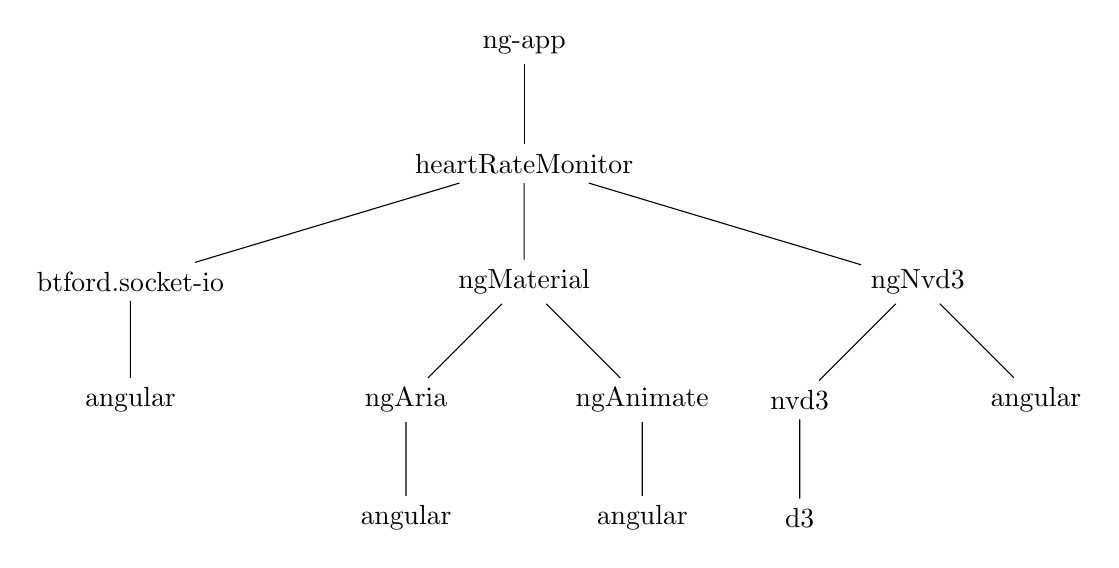
\begin{tikzpicture}[level distance=1.5cm,
	level 1/.style={sibling distance=3cm},
	level 2/.style={sibling distance=5cm},
	level 3/.style={sibling distance=3cm}]
	\node {ng-app}
	child {node {heartRateMonitor}
		child {node {btford.socket-io}
			child {node {angular}}}
		child {node {ngMaterial}
			child {node {ngAria}
				child {node {angular}}}
			child {node {ngAnimate}
				child {node {angular}}}}
		child {node {ngNvd3}
			child {node {nvd3}
				child {node {d3}}}
			child {node {angular}}}
	};
	\end{tikzpicture}
\caption{Árbol de dependencias en la aplicación Angular}
\label{figure:treeDependencies}	
\end{figure}

\begin{description}
\item[btford.socket-io] representa el módulo que integra socket.io (a su vez, otra librería JavaScript que implementa Web Sockets) dentro del mundo Angular, permitiéndonos establecer comunicaciones en tiempo real con el servidor.
\item[ngMaterial] librería que implementa el concepto visual de Diseño Material o Material Design, siguiendo las nuevas recomendaciones de diseño proporcionadas por Google. Depende a su vez de \ttw{ngAria}, la cual proporciona soporte para accesibilidad mediante la habilitación de atributos ARIA y el uso de tecnologías asistidas usadas por personas con algún tipo de discapacidad y \ttw{ngAnimate}, la cual proporciona soporte en Angular para el uso de animaciones.
\item[ngNvd3] es un módulo que permite integrar en Angular gráficas reutilizables basadas en la librería nvd3, gracias al uso de las directivas que implementa. Esta depende de d3, que es una librería para manipular documentos basados en datos, como elementos \ac{SVG}. \ttw{ngNvd3} será el módulo usado para la representación de una gráfica en tiempo real con valores de frecuencia cardíaca.
\end{description}

\subsubsection{Vista}
Una vez llevada a cabo una explicación técnica más detallada de Angular, podemos pasar a desglosar los distintos componentes del paradigma MVC, en términos de nuestra aplicación. El fragmento de código \ref{code:webHTML} representa la vista HTML de nuestra aplicación web. Cabe decir que es la única vista que contiene.

\begin{listing}[!htbp] 
%\RecustomVerbatimEnvironment{Verbatim}{BVerbatim}{}
\begin{minted}[mathescape,linenos,numberblanklines,breaklines,frame=lines]{html}
<html>
    <head>
        <!-- Titulo y carga de los archivos externos css -->
    </head>
    <body ng-controller="heartRateMonitor.controller">
        <div layout="column" layout-fill>
            <md-toolbar>
                <!-- Contenido de la barra de herramientas superior -->
            </md-toolbar>
            <md-content layout-padding layout-fill flex 
                layout="column" style="padding-top: 24px">
                <div class="heartRate-value">
                    <span style="padding-right: 10px">{{currentDay}}</span>
                    <i class="fa fa-heart-o fa-2x" style="color: pink;" 
                        ng-show="disconnected"></i>
                    <i class="fa fa-heartbeat fa-2x" style="color: #E91E63;"
                        ng-hide="disconnected"></i>
                    <span style="padding: 0px 10px 0px 10px;
                         font-size: 24px;">{{value}}</span>
               </div>
               <nvd3 options="options" data="data" 
                   config="config" api="api"></nvd3>
          </md-content>
    </div>
    <!--Punto de entrada al codigo javascript'-->
    <script type="text/javascript" 
        src="../bower_components/requirejs/require.js"
        data-main="js/main.js"></script>
    </body>
</html>
\end{minted}
\caption{Vista principal index.html}
\label{code:webHTML}
\end{listing}

El controlador Angular de nuestra aplicación se encuentra enlazado al elemento DOM \ttw{<body>}, que no es más que el cuerpo del documento HTML. Por tanto, tenemos un único controlador, \ttw{heartRateMonitor.controller}, asociado al elemento padre del contenido, que nos permitirá aplicar directivas Angular a todos sus elementos hijos, y el cual crea un nuevo ámbito o entorno de variables aisladas del entorno global, las cuales podrán ser accedidas también por los elementos hijos de las vistas usando la notación \{\{ \}\}.

Los elementos \ttw{<md-toolbar>} y \ttw{<md-content>} son elementos DOM personalizados proporcionados por la librería \ttw{ngMaterial}, los cuales permiten configurar fácilmente la predisposición de los elementos en la barra de acción y contenido mediante atributos HTML, los cuales serán compilados a código CSS.
Las variables enlazadas \ttw{currentDay} y \ttw{value} representan respectivamente la fecha actual y el valor de frecuencia cardíaca recibido en cada momento.
El elemento \ttw{nvd3} es otro elemento DOM personalizado agregado por la librería \ttw{ngNvd3}, el cual representa la gráfica de tipo \tit{line-chart} o gráfica de línea, que usaremos para mostrar los últimos valores recibidos de frecuencia cardíaca, así como el actual.
Por último la etiqueta \ttw{<script>} es el único script necesitado en nuestro HTML, actuando como el punto de entrada que la librería RequireJS necesita, para efectuar así la construcción del árbol de dependencias previo al arranque de AngularJS.

\subsubsection{Controlador y modelo}
El controlador y subsecuente modelo de objetos se encuentran definidos en el archivo \ttw{heartRateMonitor-controller.js}. En él se alberga toda la lógica Javascript del lado del cliente, como las opciones, configuración y datos de la gráfica, los cuales se definen mediante objetos JSON.

También se encuentra el manejo de la conexión socket del lado del cliente, de forma que el controlador se encuentra subscrito a dos eventos. El primero de ellos es la llegada de nuevos valores de frecuencia cardíaca provenientes del servidor. Cuando esto ocurre se añade el nuevo valor al final de la gráfica y se elimina el valor más antiguo, simulando un comportamiento de tiempo real, ya que la gráfica transmite la sensación de ir desplazándose con el tiempo. El segundo de ellos es la llegada de un nuevo valor de localización. Esto permitirá al usuario acceder a la ubicación actualizada en un mapa mediante el pulsado del botón ``Localización'' pertinente.

Por último decir que el controlador también se encarga de manejar el dinamismo de la página en cuanto a cambios de tamaño de pantalla se refiere. De esta forma, si estamos en un ordenador portátil típico con monitor de 15 pulgadas y tenemos el navegador en pantalla completa, mostraremos 10 muestras en la gráfica, mientras que si nos encontramos en un dispositivo móvil, como puede ser un teléfono inteligente de 4 pulgadas, mostraremos 2 o 4 muestras, en función de la orientación de este. Esto se verá reflejado en el siguiente capítulo.

\chapterend{}